\documentclass[sigconf]{acmart}

\usepackage{booktabs} % For formal tables
\usepackage{graphicx}
\usepackage{balance}  % for  \balance command ON LAST PAGE  (only there!)
\usepackage{amssymb}
\usepackage{graphicx}
\usepackage{float}
\usepackage{subfigure}
\usepackage{mathtools}
\usepackage{eurosym}

\usepackage{pgfplots}
\usepackage{url}
\usepackage{enumitem}
\usepackage[linesnumbered,ruled]{algorithm2e}
\usepackage[export]{adjustbox}
\usepackage{xspace}
\usepackage{breqn}

% Copyright
%\setcopyright{none}
%\setcopyright{acmcopyright}
%\setcopyright{acmlicensed}
\setcopyright{rightsretained}
%\setcopyright{usgov}
%\setcopyright{usgovmixed}
%\setcopyright{cagov}
%\setcopyright{cagovmixed}


% DOI
\acmDOI{10.475/XXX_X}

% ISBN
\acmISBN{XXX-XXX-XX-XXX/10/18}

%Conference
\acmConference[CIKM'18]{ACM International Conference on Information and Knowledge Management}{October 2018}{
  Lingotto, Turin Italy}
\acmYear{2018}
\copyrightyear{2018}


\acmArticle{4}
\acmPrice{15.00}

% These commands are optional
%\acmBooktitle{Transactions of the ACM Woodstock conference}
\editor{Rakesh Agrawal}
\editor{Andrei Broder}
\editor{Mohammed Zaki}


\begin{document}
\title{Exploration of Interesting Dense Regions on Spatial Data}
%\titlenote{Produces the permission block, and
%  copyright information}
%\subtitle{Extended Abstract}
%\subtitlenote{The full version of the author's guide is available as
%  \texttt{acmart.pdf} document}

\author{Double-blind submission}

% \author{Behrooz Omidvar-Tehrani}
%\affiliation{%
  %\institution{University of Grenoble Alpes (France)}
%}
%\email{behrooz.omidvar-tehrani@univ-grenoble-alpes.fr}

%\author{Pl\'acido A. Souza Neto}
%\affiliation{%
 % \institution{Federal Institute of Rio Grande do Norte (Brazil)}
%}
%\email{placido.neto@ifrn.edu.br}


%\author{Francisco B. Silva J\'unior}
%\affiliation{%
%\institution{Federal Institute of Rio Grande do Norte (Brazil)}
%}
%\email{bento.francisco@academico.ifrn.edu.br}	

%\author{Felipe F. Pontes}
%\affiliation{%
%\institution{Federal Institute of Rio Grande do Norte (Brazil)}
%}
%\email{freire.pontes@academico.ifrn.edu.br}


%\author{Tiago Oliveira Lisboa}
%\affiliation{%
% \institution{Federal Institute of Rio Grande do Norte (Brazil)}
%}
%\email{tiago.oliveira@academico.ifrn.edu.br}



% The default list of authors is too long for headers.
%\renewcommand{\shortauthors}{B. Trovato et al.}


\begin{abstract}
The large size of spatial data hinders its effective analysis for discovering insights. Analysts require to obtain only few options (so-called ``highlights'') to focus on. In this paper, we define, formalize and analyse the concept of interesting dense regions (IDR) in order to find possible preferred regions to the analyst. The objective is to obtain one or several regions in which the analyst has expressed her implicit feedback. Our proposal consider a polygon-based abstraction layer for captured interactions. Using these interesting dense regions, we highlight points to guide the analysis process. We also analyse its efficiency and effectiveness through a realistic example.
\end{abstract}

%
% The code below should be generated by the tool at
% http://dl.acm.org/ccs.cfm
% Please copy and paste the code instead of the example below.
%
%\begin{CCSXML}
%<ccs2012>
 %<concept>
  %<concept_id>10010520.10010553.10010562</concept_id>
  %<concept_desc>Computer systems organization~Embedded systems</concept_desc>
  %<concept_significance>500</concept_significance>
 %</concept>
 %<concept>
  %<concept_id>10010520.10010575.10010755</concept_id>
  %<concept_desc>Computer systems organization~Redundancy</concept_desc>
  %<concept_significance>300</concept_significance>
 %</concept>
 %<concept>
  %<concept_id>10010520.10010553.10010554</concept_id>
  %<concept_desc>Computer systems organization~Robotics</concept_desc>
  %<concept_significance>100</concept_significance>
 %</concept>
 %<concept>
 % <concept_id>10003033.10003083.10003095</concept_id>
  %<concept_desc>Networks~Network reliability</concept_desc>
  %<concept_significance>100</concept_significance>
 %</concept>
%</ccs2012>
%\end{CCSXML}

%\ccsdesc[500]{Computer systems organization~Embedded systems}
%\ccsdesc[300]{Computer systems organization~Redundancy}
%\ccsdesc{Computer systems organization~Robotics}
%\ccsdesc[100]{Networks~Network reliability}


\keywords{Dense regions, highlight, IDR, spatial data, implicit feedback.}


\maketitle



\section{Introduction}



Spatial data are often voluminous. Hence the focus in the literature of spatial data analysis is on ``efficiency'', i.e., enabling fluid means of navigation in spatial data to facilitate the exploratory analysis. The common approach is to design pre-computed indexes which enable efficient retrieval of spatial data (e.g., \cite{lins2013nanocubes}). However, there has been fewer attention to the ``value'' derived from spatial data. Despite the huge progress on the efficiency front, an analyst may easily get lost in the plethora of geographical points due to two following reasons.

\vspace{3pt}
\noindent $\blacksquare$ In an exploratory context, the analyst doesn't know apriori what to investigate next.

\vspace{2pt}
\noindent $\blacksquare$ Moreover, she may easily get distracted and miss interesting points by visual clutter caused by huge point overlaps.

\vspace{3pt}
The main drawback of the traditional analysis model is that the analyst has a {\em passive role} in the process. In other words, the analyst's feedback~\cite{kamat2014distributed,Omidvar-Tehrani:2015} (i.e., her likes and dislikes) is ignored and only the input query (i.e., her explicit request) is served. In case feedback is incorporated, the process can be more directed towards analyst's interests where her partial needs can be served earlier in the process. In this paper, we advocate for a ``guidance layer'' on top of the raw visualization of spatial data to enable analysts know {\em ``what to see next''}. This guidance should be a function of analyst feedback: the system should recommend options similar to what the analyst has already appreciated. 
 
Considering this context, we propose in this paper an approach to explore Interesting Dense Regions (IDRs)  whose aim is to capture and analyze implicit feedback of analysts in spatial data analysis. Without loss of generality, we focus on ``mouse moves'' as the implicit feedback received from the analyst. Mouse moves are the most common way that analysts interact with geographical maps~\cite{Chen:2001}.  However, our approach can be easily extended to other types of inputs such gaze tracking, leap motions, etc.

% K-DBSCAN with the main focus of identifying clusters of points with similar spatial density.  K-DBSCAN lies in finding arbitrary shaped clusters in variable density regions. Moreover, it can also discover clusters with overlapping spatial regions, but differing density levels.
 
 
\section{Interesting Dense Regions}


An Interesting Dense Region (\textit{IDR}) is a region with high possibility to have a set of point that may be interesting to the analyst. An IDR is captured and defined by processing user feedbacks. Unlike the literature which mainly focuses on explicit feedback, we investigate on implicit feedback. There are different ways to capture implicit feedbacks: (\textit{i}) During spatial data analysis, it is often the case that analysts look at some regions of interest but forget to provide an explicit feedback. We call this latent signal, gaze. It shown in [5] that gaze has a strong correlation with ``user attention''. The signal can be captured by tracking eye movements \citep{arapakis2014user}; (\textit{ii}) To address privacy issues of web-cam exploitation for gaze tracking, we consider an alternative option of tracking the mouse cursor. It is shown in \cite{arapakis2014understanding} that mouse gestures have a strong correlation with ``user engagement''. Intuitively, a point receives a positive feedback if the cursor moves around it frequently. (\textit{iii}) In most spatial datasets, there is a profile page dedicated to each point.  We consider the amount of time that the analyst spends in a page as an implicit feedback. For instance, if the analyst spends few minutes in a page for an apartment with balcony in center of Paris, this counts as positive feedback for this type of apartment. So, the objective of IDR's definition is to obtain one or several regions in which the analyst has expressed her implicit feedback. 

There are two observations for such regions definition:

\vspace{2pt}
\noindent $\blacksquare$ {\bf Observation 1.} We believe that a region appeals more interesting to the analyst if it is denser, i.e., the analyst moves her mouse in that region several times.

\vspace{2pt}
\noindent $\blacksquare$ {\bf Observation 2.} It is possible that the analyst moves her mouse everywhere in the map. This should not signify that everywhere in the map has the same significance.

We consider two different layers on a geographical map: ``spatial layer'' and ``interaction layer''. The spatial layer contains points from a spatial database $\mathcal{P}$. The interaction layer contains mouse move points $\mathcal{M}$.

Our proposal algorithm mines a set of mouse move points $\mathcal{M}$ in the interaction layer to discover one or several Interesting Dense Regions, in which most analyst's interactions occur. Then it matches the spatial points $\mathcal{P}$ with IDRs  in order to find points inside each region. The attributes of resulting points will be exploited to update a analyst's feedback vector. The updated vector $F$ will then be used to find $k$ highlights. These steps ensure that the final highlights reflect analyst's implicit interests. 

Following our observations, we propose Algorithm \ref{algo:dense} for mining IDRs. We add points to $\mathcal{M}$ only every $200ms$ to prevent adding redundant points.  Following Observation 1 and in order to mine the recurring behavior of the analyst, the algorithm begins by partitioning the set $\mathcal{M}$ into $g$ fixed-length consecutive segments $\mathcal{M}_0$ to $\mathcal{M}_g$. The first segment starts at time zero (where the system started), and the last segment ends at $t_c$, i.e., the current time. Following Observation 2, we then find dense clusters in each segment of $\mathcal{M}$ using a variant of DB-SCAN~\cite{Ester:1996} approach. Finally, we return intersections among those clusters as IDRs.




\begin{algorithm}[t]
\DontPrintSemicolon
\KwIn{Current time $t_c$, mouse move points $\mathcal{M}$}
\KwOut{IDRs $\mathcal{S}$}
$\mathcal{S} \gets \emptyset$\;
$g \gets ${\em number of time segments}\;
\For{$i \in [0,g]$}
{
       $\mathcal{M}_i \gets \{m = \langle x,y,t \rangle | (\frac{t_c}{g} \times i) \leq t \leq (\frac{t_c}{g} \times (i+1))\}$\;
       $\mathcal{C}_i \gets \mathit{mine\_clusters}(\mathcal{M}_i)$\label{ln:mine}\;
       $\mathcal{O}_i \gets \mathit{find\_ploygons}(\mathcal{C}_i)$\label{ln:poly}\;
}
\lFor{$\mathcal{O}_i, \mathcal{O}_j$ where $i,j \in [0,g]$ and $i \neq j$}
{
       $\mathcal{S}.\mathit{append}(\mathit{intersect}(\mathcal{O}_i, \mathcal{O}_j))$
}
\Return{$\mathcal{S}$}\; 
\caption{Find Interesting Dense Regions (IDRs)}
\label{algo:dense}
\end{algorithm}


\vspace{2pt}
For clustering points in each time segment (i.e., line \ref{ln:mine} of Algorithm~\ref{algo:dense}), we use ST-DBSCAN~\cite{Birant:2007}, a space-aware variant of DB-SCAN for clustering points based on density. For each subset of mouse move points $\mathcal{M}_i$, $i \in [0,g]$, ST-DBSCAN begins with a random point $m_0 \in \mathcal{M}_i$ and collects all density-reachable points from $m_0$ using a distance metric. As mouse move points are the 2-dimensional pixel space (i.e., the display), we choose euclidean distance as the distance metric. If $m_0$ turns out to be a core object, a cluster will be generated. Otherwise, if $m_0$ is a border object, no point is density-reachable from $m_0$ and the algorithm picks another random point in $\mathcal{M}_i$. The process is repeated until all of the points have been processed.

\vspace{2pt}
Once clusters are obtained for all subsets of $\mathcal{M}$, we find their intersections to locate recurring regions (line \ref{ln:poly}). To obtain intersections, we need to clearly define the spatial boundaries of each cluster. Hence for each cluster, we discover its corresponding polygon that covers the points inside. For this aim, we employ Quickhull algorithm, a quicksort-style method which computes the convex hull for a given set of points in a 2D plane~\cite{Barber:1996}.

There exist several approaches to infer a spatial region for a given set of points \cite{Bevis1989,DUCKHAM2008,FADILI2004,ARAMPATZIS2006,Galton2006}. The common approach is to cluster points in form of concave and convex polygons.  In case a concave polygon is constructed, the ``dents'' of such a polygon may entail points which are not necessarily in $\mathcal{M}$. In IDR algorithm, however, we adapt Quickhull~\cite{Barber:1996}, due its simplicity, efficiency and it's natural implementation of convex polygons.

\section{Case Study and Experiments}

This section describes an example to guide the experiments made over the proposal presented in this paper. The following use case describes a scenario of implicit feedbacks. 


\begin{figure*}[t]
\centering
   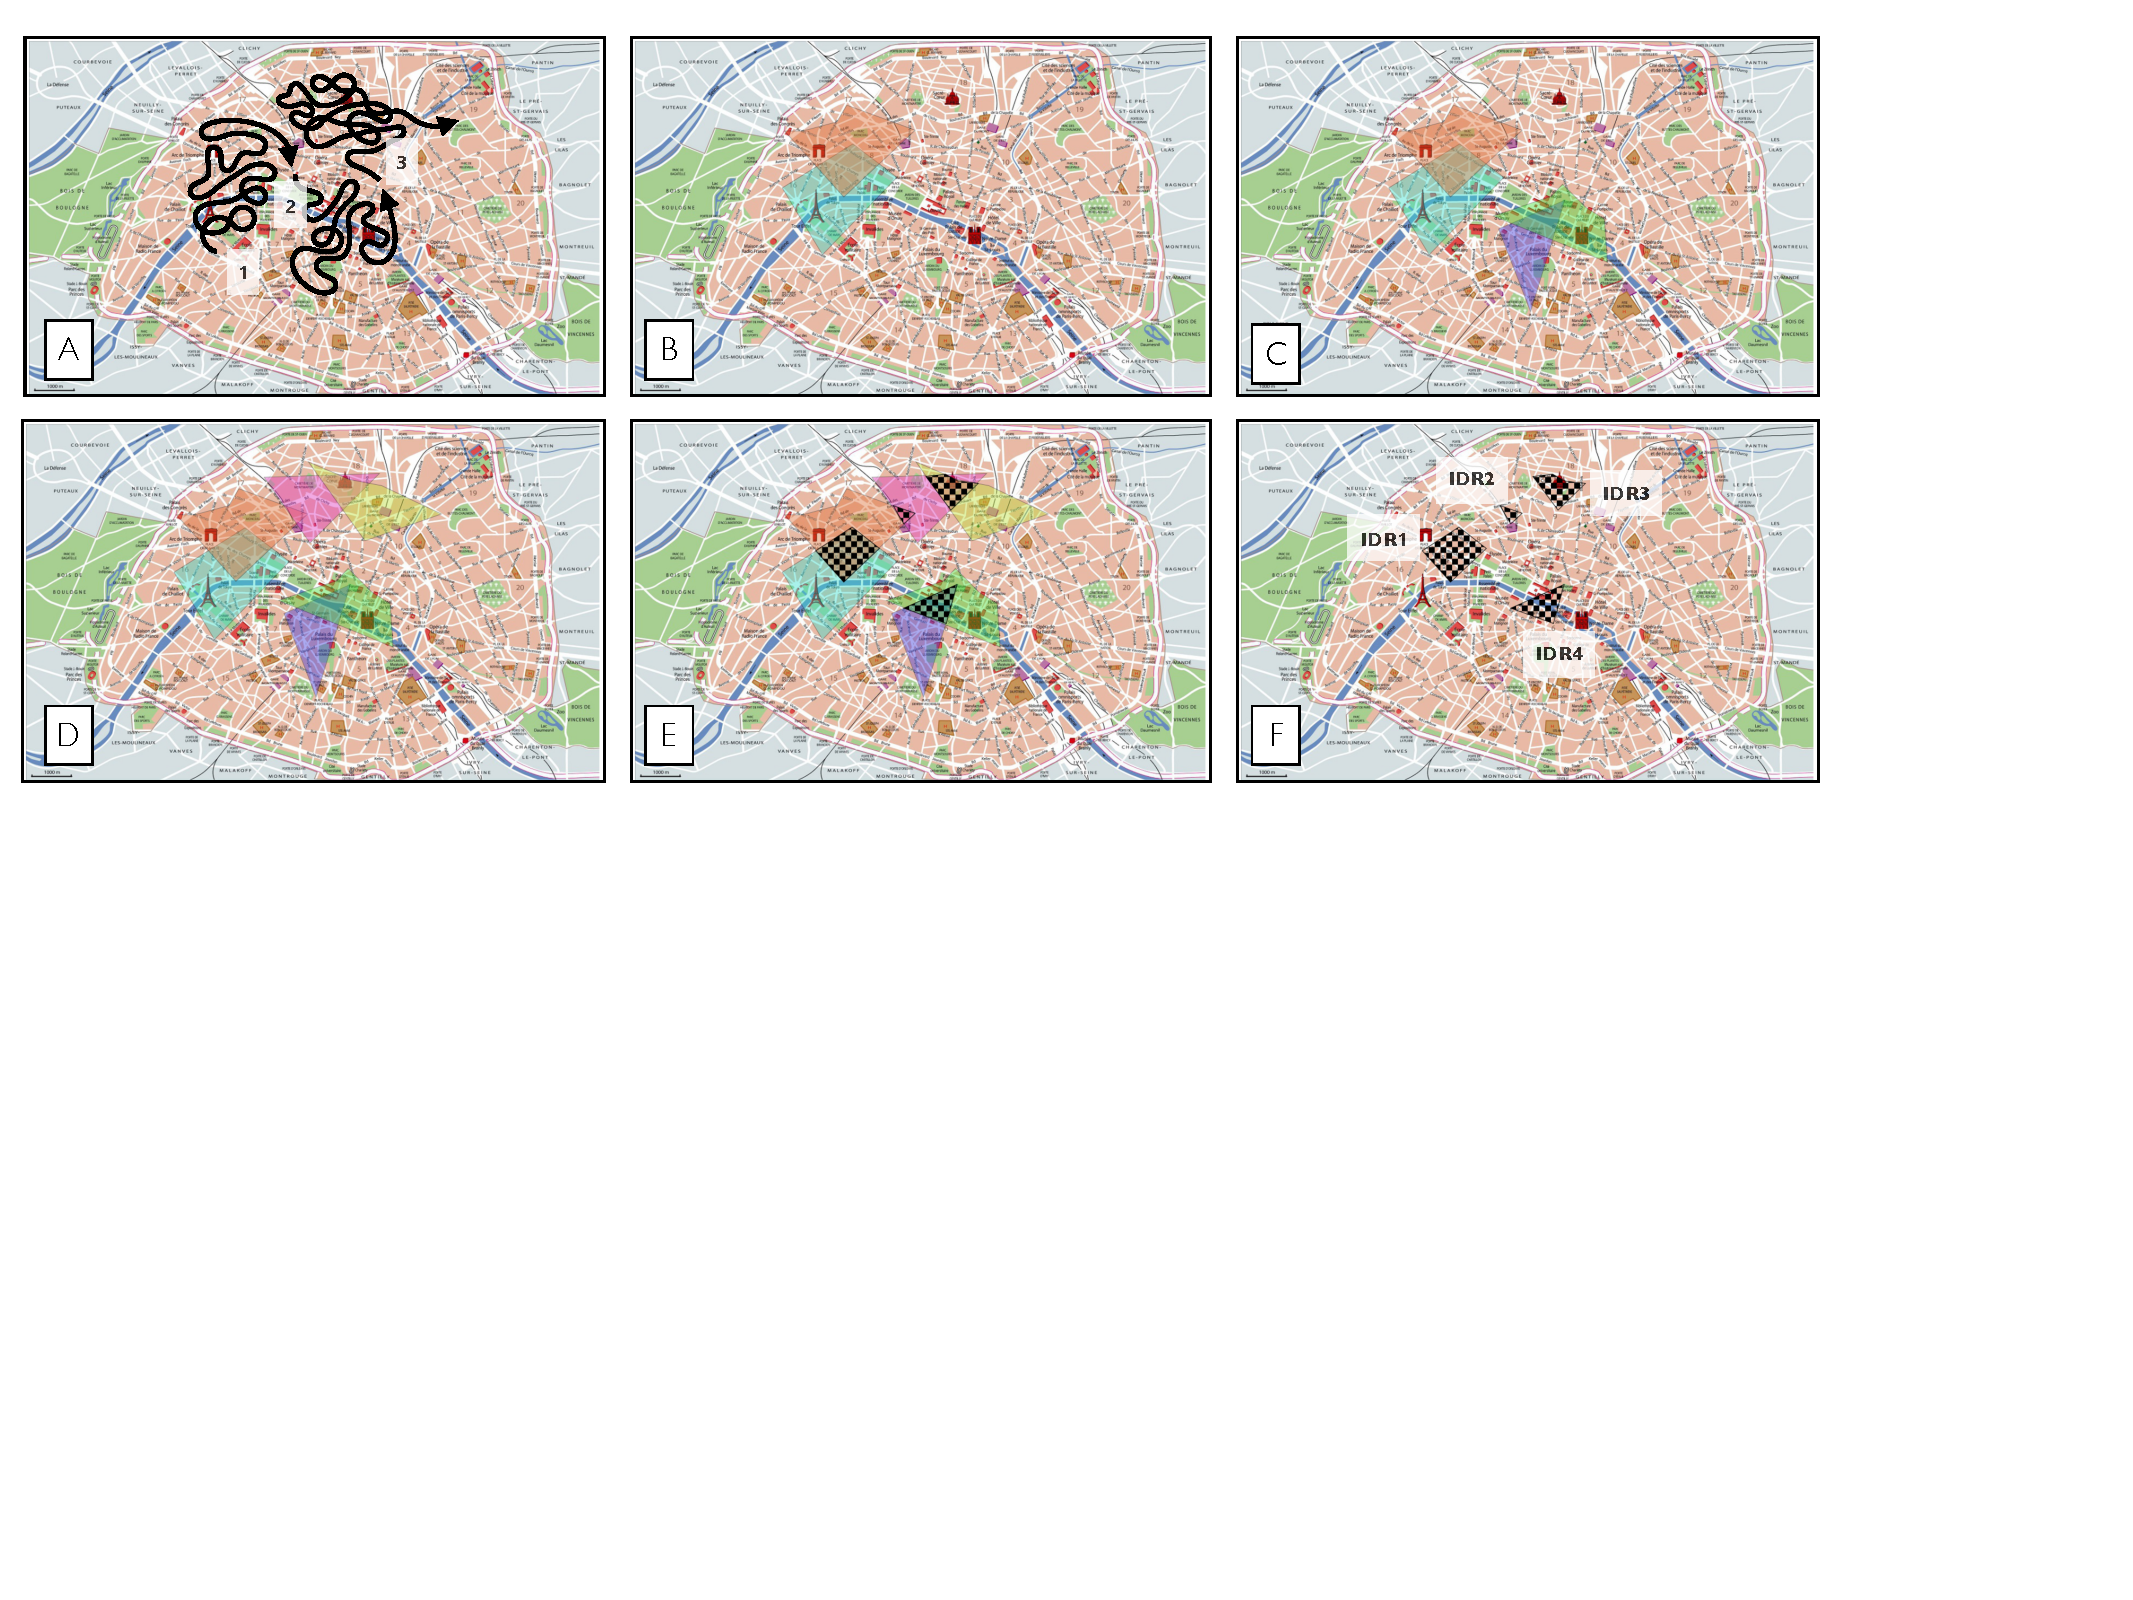
\includegraphics[width=\textwidth]{imgs/regions}
  \caption{The process of finding IDRs - Paris city.}
  \label{fig:regions}
\end{figure*}



\begin{figure}[t]
\centering
   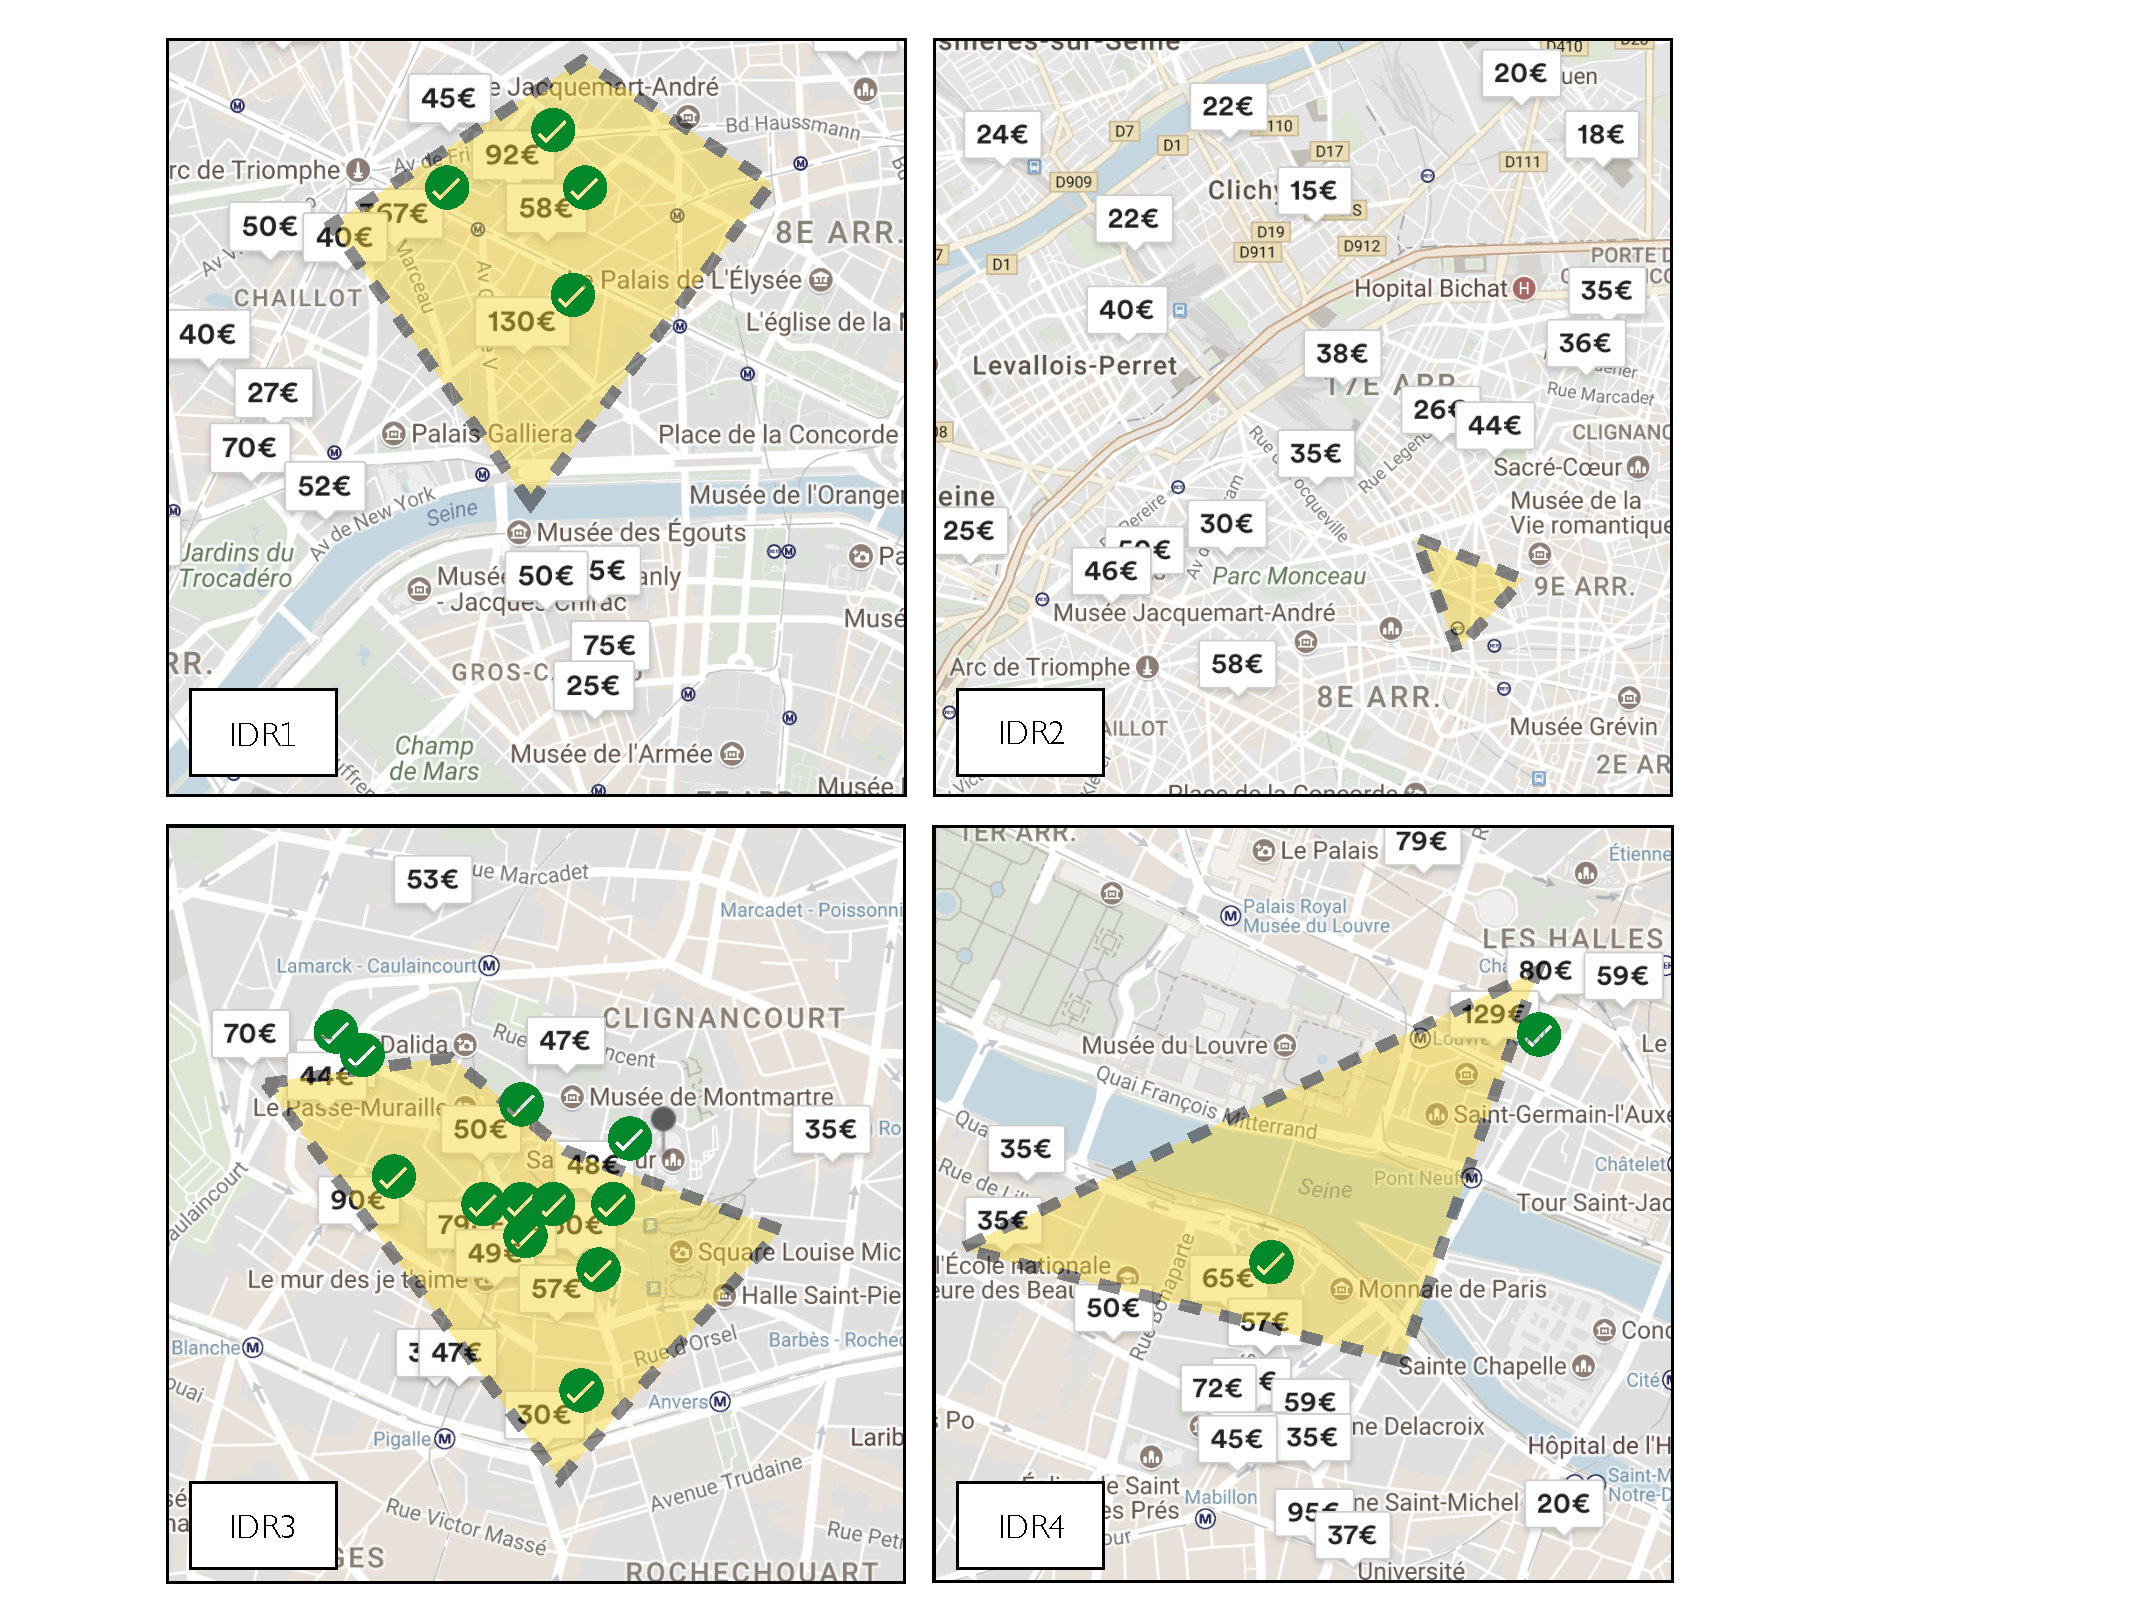
\includegraphics[width=\columnwidth]{imgs/match}
  \caption{Matching points for IDRs.}
  \label{fig:match}
\end{figure}

\vspace{2pt}
\noindent {\bf Example.} {\em Lucas is planning to pass some days in Paris, France. He loves French culture and language, and pass some days in a nice city would be delighted to him.  He decides to rent a home-stay from Airbnb website\footnote{\it http://www.airbnb.com}. He likes to discover the city, hence he is open to any type of lodging in any region with an interest to stay in the city center. The website returns 4000 different locations. As he has no other preferences, an exhaustive investigation needs scanning each location independently which is nearly infeasible. While he is scanning few first options, he shows interest in the region of \textit{Champ de Mars} (close to Eiffel Tower), but he forgets or doesn't feel necessary to click a point there. An ideal system should capture this implicit feedback in order to short-list a small subset of locations that Lucas should consider as high priority}.

We describe the process of finding IDRs in an example. Figure \ref{fig:regions} shows the steps that Lucas follows in our running example to explore home-stays in Paris. Figure \ref{fig:regions}.A shows mouse movements of Lucas in different time stages. In this example, we consider $g = 3$ and capture Lucas feedback in three different time segments (progressing from Figures \ref{fig:regions}.B to \ref{fig:regions}.D). It shows that Lucas started his search around Eiffel Tower and Arc de Triomphe (Figure \ref{fig:regions}.B) and gradually showed interest in south (Figure \ref{fig:regions}.C) and north (Figure \ref{fig:regions}.D) as well. All intersections between those clusters are discovered (hatching regions in Figure \ref{fig:regions}.E) which will constitute the set of IDRs (Figure \ref{fig:regions}.F), i.e., IDR1 to IDR4.


In the Airbnb dataset points are home-stays which are shown with their nightly price on the map. We observe (Figure \ref{fig:match}) that there exist many matching points with IDR3 and absolutely no matching point for IDR2. For IDR4, although there exist many home-stays below the region, we never check their containment, as they belong to a Quadtree cell which doesn't intersect with the IDR. 

Considering the described example we perform two sets of experiments. A first set of few experiments to validate its efficiency and effectiveness. The second set of experiments aims to analyse the number of IDRs generated for each interaction, the number of points and its percentage highlighted from the dataset. In the interest of space, we only present a glimpse of our experiments here. More will be discussed in an extended version. 

\vspace{2pt}
First off, we validate the ``usability'' of our proposal. For this aim, we design a user study with some participants who are all students of Computer Science. Some of them are ``novice'' users who don't know the location, and some are ``experts''. Participants should fulfill a task. For each participant, we report a variant of time-to-insight measure, i.e., how long the participants interact with the frameworks before fulfilling the task. Evidently, less number of interactions is preferred as it means that the participant can reach insights faster. Then we measure the time to execute the task.


\vspace{2pt}
On the Airbnb dataset of Paris with 1,000 points, we define two different tasks: {\em T1: ``finding a point in a requested location''} (e.g., find a home-stay in the ``\textit{Champ de Mars}'' area), and {\em T2: ``finding a point with a requested profile''} (e.g., find a cheap home-stay.) Participants may also begin their navigation either from {\em I1: ``close to the goal''} or {\em I2: ``far from the goal''}. 


\begin{table}[h]
\centering
\caption{``Novice'' and ``Experts'' - Interactions (in seconds)}
\label{tbl:novice}
\begin{tabular}{c|c|c|c|c|}
\cline{2-5}
                                       	& \textbf{T1/I1} 	& \textbf{T2/I1} 	& \textbf{T1/I2}	& \textbf{T2/I2}	\\ \hline
\multicolumn{1}{|c|}{Novices} 				& 1.99            	& 2.38	          	& 2.00              & 2.48              \\ \hline
\multicolumn{1}{|c|}{Experts} 				& 1.72            	& 2.09	          	& 1.70              & 2.14              \\ \hline
\end{tabular}
\end{table}


\vspace{2pt}
Participants benefit from information highlighting based on their implicit feedback. Table \ref{tbl:novice} reports the time for the interactions to find what they are looking for, novice and expert participants, respectively. We observe that on average the system spends $2.067$ seconds to return a defined goal. This shows that implicit feedback capturing is an effective mechanism which helps analysts to reach their goals faster.

\vspace{2pt}
Expert participants need $0.35$ (seconds) fewer interactions on average. Interestingly, starting points, i.e., {\em I1} and {\em I2}, do not have a huge impact on number of steps. It is potentially due to the diversity component which provides distinct options and can quickly guide analyst towards their region of interest. We also observe that the task {\em T2} is an easier task than {\em T1}. This is potentially due to  where the analyst can request options similar to what she has already observed and greedily move to her preferred regions.

\vspace{6pt}
The second set of experiments consider 2 different datasets, Airbnb~\footnote{https://www.airbnb.com/ and http://insideairbnb.com/get-the-data.html} and Yelp~\footnote{https://www.yelp.com/} datasets with spatial points in Paris city, apartment and restaurant datasets, respectively.  For each type of dataset we proceed the experiments with 4 volume of points, 100, 1000, 2000 and 4000 points, respectively. For each volume of points we proceed 20 interactions, and we present the results averages.  So, we proceed 80 interactions using the Airbnb dataset and 80 interactions using the Yelp dataset.

We pass 2 minutes trying to find an interesting point, in each interact. We capture, in each interaction, the following informations: (i) the number of regions created from the mouse movements during the interactions; (ii) the number of IDRs (intersection of regions) generated after the interactions; (iii) the number of points from the dataset presented in each IDR after the interaction; and finally (iv) the percentage of points (from the dataset volume) inside the IDRs.  

In this set of experiment we validate not only the ``usability'' of our proposal, but also we analyse how the IDRs are generated and the how many interesting regions and points can be highlighted from the implicit feedbacks captured during the user interactions. Tables \ref{tbl:airbnb} and \ref{tbl:yelp} present the result for each dataset. 

For the apartment dataset experiments (Table \ref{tbl:airbnb}) the number of regions decreases while the number of points increases. The general average of regions created is around 10, per interaction. The same happens for IDRs, except when we have 4000 points. The average of points presented in IDRs is 24.97. So, the system is able to highlight at least  8.05\% of point from the dataset, in average. 

\begin{table}[h]
\centering
\caption{Airbnb dataset - Paris city}
\label{tbl:airbnb}
\begin{tabular}{|c|c|c|c|c|}
\cline{1-5}
\textbf{n. points}  & \textbf{regions} 	& \textbf{IDRs} 	& \textbf{points in IDRs}	& \textbf{\%  points}	\\ \hline
\multicolumn{1}{|c|}{100} 				& 11.35            	& 10.05	          	& 29.40             & 29.40\%            
 \\ \hline
\multicolumn{1}{|c|}{1000} 				& 10.75          	& 6.75	          	& 11.70              & 1.17\%              \\ \hline
\multicolumn{1}{|c|}{2000} 				& 7.37           	& 3.63         	& 5.63             & 0.003\%              \\ \hline
\multicolumn{1}{|c|}{4000} 				& 10.30           	& 10.15	          	& 53.15              & 1.33\%              \\ \hline
\multicolumn{1}{|c|}{\textbf{average}} 				& \textbf{9.94}           	& \textbf{7.64}	          	&\textbf{ 25.97}              & \textbf{8.05\% }             \\ \hline

\end{tabular}
\end{table}

The results for the restaurant dataset (Table \ref{tbl:yelp}) is more uniform than the one presented in Table \ref{tbl:airbnb}. The general average of regions created is 12.75 regions per interaction. The number of regions also decreases while the number of points increases.  The same happens for IDRs, where we have an average of 8.9 IDRs generated per interaction.  The number of points presented in IDRs is 108.65, in average, and it represents 13.11\% of points  highlighted from the dataset, in average. 

For both datasets we considered the location presented in our example scenario, where Lucas is planning to pass some vacations days in Paris. 


\begin{table}[h]
\centering
\caption{Yelp dataset - Paris city}
\label{tbl:yelp}
\begin{tabular}{|c|c|c|c|c|}
\cline{1-5}
\textbf{n. points}  & \textbf{regions} 	& \textbf{IDRs} 	& \textbf{points in IDRs}	& \textbf{\%  points}	\\ \hline
\multicolumn{1}{|c|}{100} 				& 14.90            	& 7.55	          	& 28.30             & 28.30\%            
 \\ \hline
\multicolumn{1}{|c|}{1000} 				& 13.90         	& 10.00	          	& 149.55             & 14.96\%              \\ \hline
\multicolumn{1}{|c|}{2000} 				& 11.05         	& 9.80         	& 111.05             & 5.55\%              \\ \hline
\multicolumn{1}{|c|}{4000} 				& 10.45          	& 8.55	          	& 145.7              & 3.64\%              \\ \hline
\multicolumn{1}{|c|}{\textbf{average}} 				& \textbf{12.57}           	& \textbf{8.97}	          	& \textbf{108.65}              & \textbf{13.11\%}              \\ \hline
\end{tabular}
\end{table}


\section{Conclusions}

In this paper, we propose to explore Interesting Dense Regions (\textit{IDRs}) of spatial information highlighting using implicit feedback. The implicit feedbacks are captured from mouse movements of the analyst over the geographical map. We formulate and formalize a novel polygon-based capturing algorithm which returns few highlights (regions) in line with analyst's implicit preferences. 

\vspace{2pt}
We consider some directions of improvement for this work. We are interested to incorporate an ``explainability'' component  which can describe causalities behind preferences. For instance, we are interested to find seasonal patterns to see why the preferences of analysts change from place to place during various seasons of the year. Another direction is to incorporate ``Query by Visualization'' approaches, where analysts can specify their intents alongside their implicit preferences, directly on the map \cite{siddiqui2016effortless}.

\bibliographystyle{ACM-Reference-Format}
\bibliography{main}

\end{document}
